\documentclass{standalone}
\usepackage{pgfplots}
\usepackage{lmodern}
\pgfplotsset{compat=1.17}

\begin{document}
	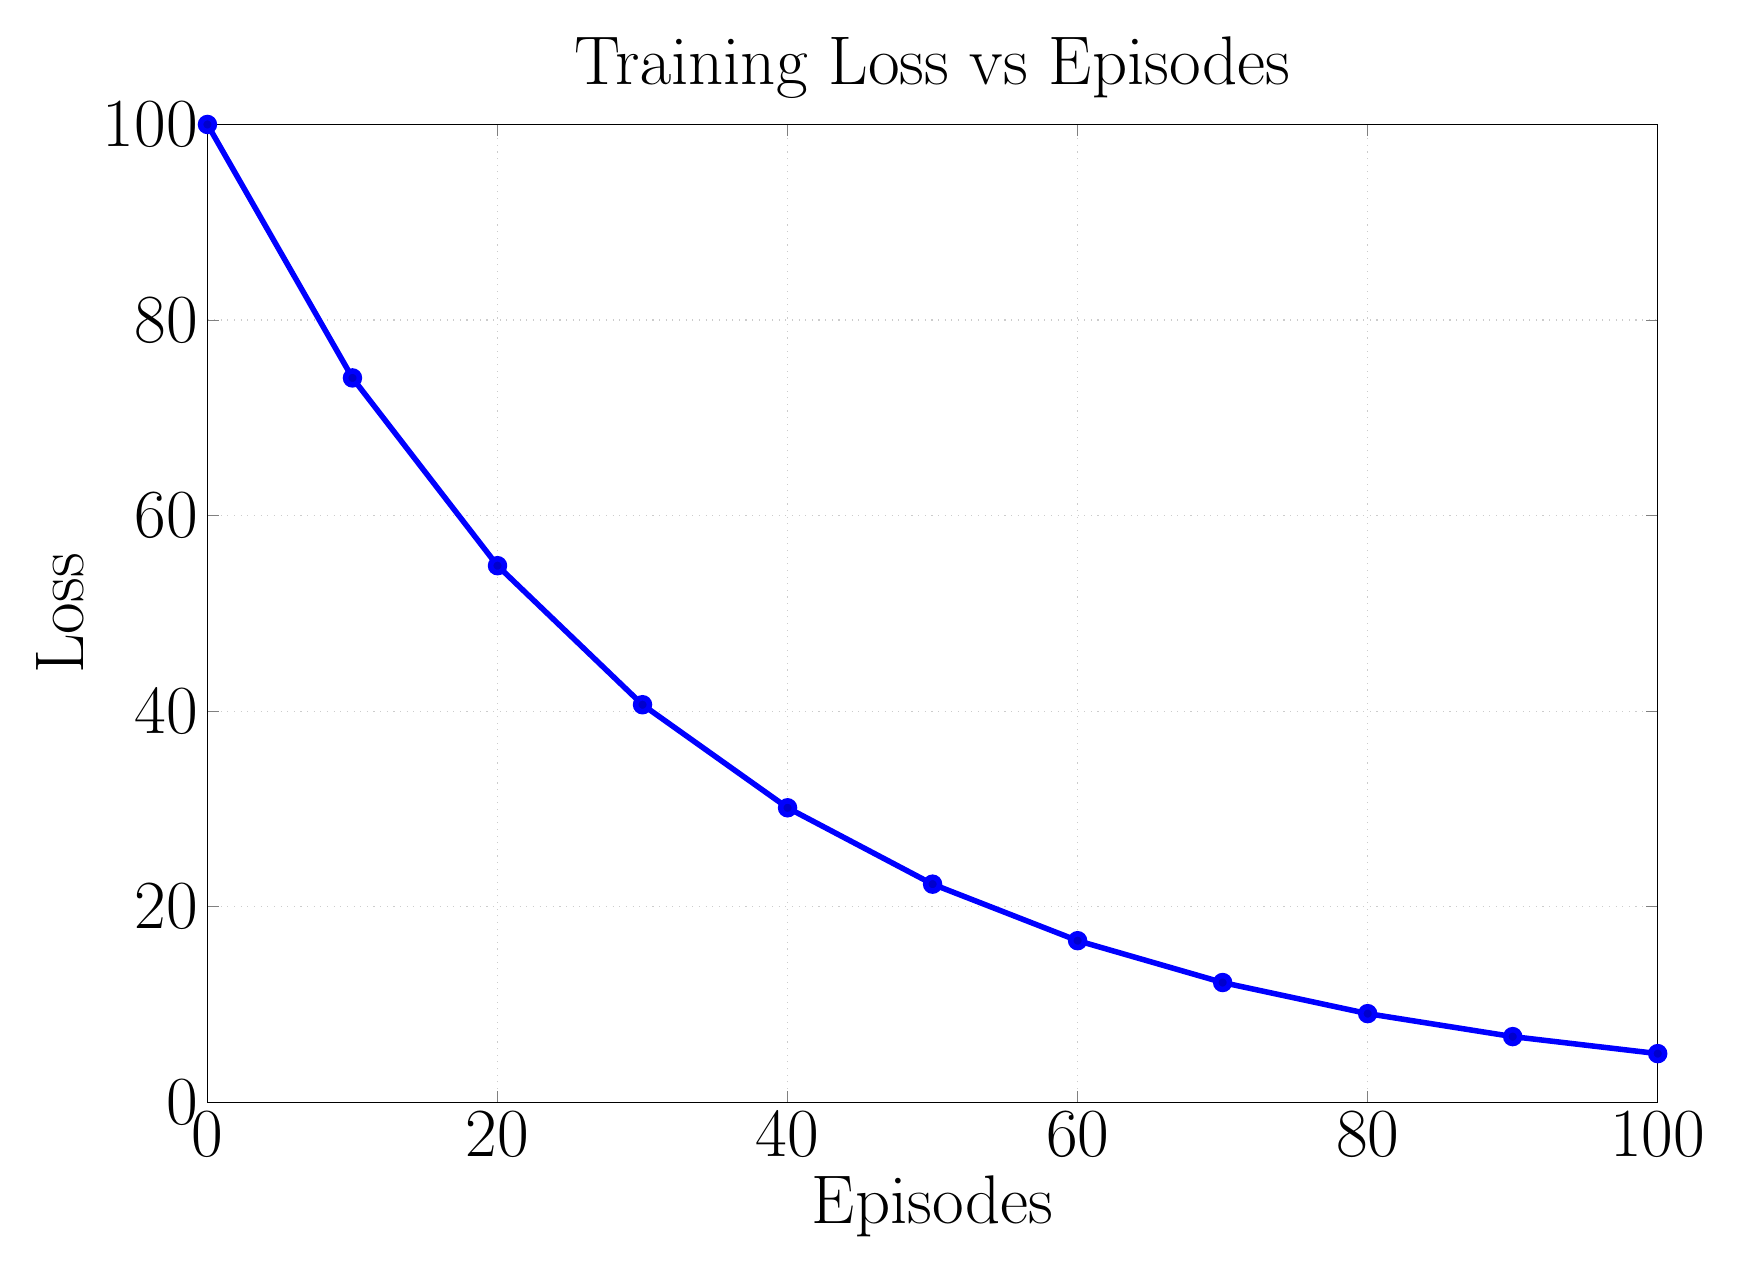
\begin{tikzpicture}
		\begin{axis}[
			width=20cm,
			height=14cm,
			tick label style={font=\fontsize{24}{28}\selectfont},
			label style={font=\fontsize{24}{28}\selectfont},
			title style={font=\fontsize{24}{28}\selectfont},
			xlabel={Episodes},
			ylabel={Loss},
			title={Training Loss vs Episodes},
			xmin=0, xmax=100,
			ymin=0, ymax=100,
			xtick={0,20,40,60,80,100},
			ytick={0,20,40,60,80,100},
			grid=both,
			grid style={dotted, gray!40},
		]
			
			\addplot+[mark=*, color=blue, line width=2pt, mark size=2.5pt] coordinates {
				(0,100)(10,74.08)(20,54.88)(30,40.66)(40,30.12)(50,22.31)(60,16.53)(70,12.25)(80,9.07)(90,6.72)(100,4.98)
			};
			
		\end{axis}
	\end{tikzpicture}
\end{document}
